
\begin{question}
Please make a frequency table and a frequency histogram from the
following (unsorted) continuous data by rounding to the nearest integer.

\begin{longtable}[]{@{}rrrrrr@{}}
\toprule
\endhead
45.2712 & 44.1466 & 43.2676 & 43.8918 & 44.0346 & 45.8148\tabularnewline
47.1033 & 44.2204 & 44.3449 & 45.9275 & 44.4923 & 45.8552\tabularnewline
43.0629 & 45.1925 & 46.1901 & 42.4973 & 43.4716 & 46.6429\tabularnewline
43.5419 & 47.0171 & 43.4011 & 44.6069 & 47.0484 & 43.7841\tabularnewline
\bottomrule
\end{longtable}
\end{question}

\begin{solution}
Make a frequency table.

\begin{longtable}[]{@{}rr@{}}
\toprule
bin & frequency\tabularnewline
\midrule
\endhead
42 & 1\tabularnewline
43 & 4\tabularnewline
44 & 8\tabularnewline
45 & 3\tabularnewline
46 & 4\tabularnewline
47 & 4\tabularnewline
\bottomrule
\end{longtable}

Make the histogram.

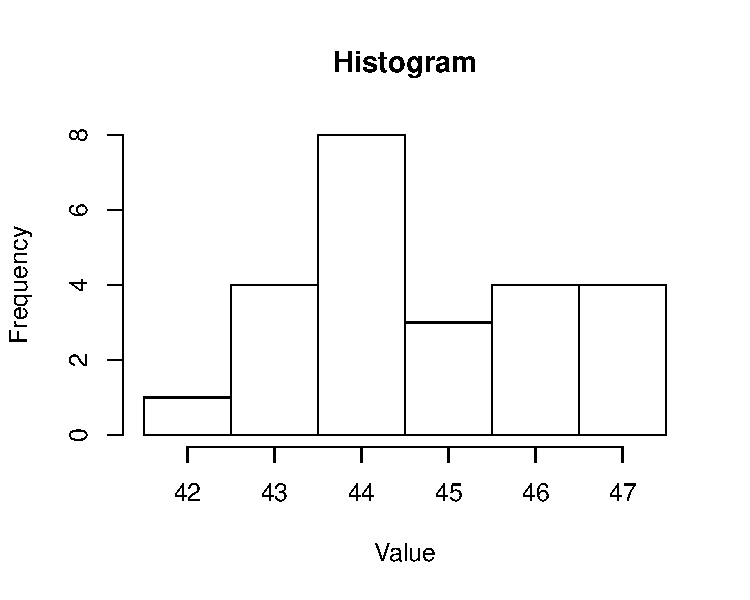
\includegraphics{barchart-1-5.pdf}\\
\end{solution}

